\chapter{Algorytm}
\label{cha:Algorytm}

\newpage
\section{Umiejscowienie znaków na drodze}
\label{sec:speedLimitLocalization}
Znaki drogowe ograniczenia prędkości są ustawione według następujących kryteriów:
\begin{itemize}
\item na początku każdej drogi
\item przed nieoznakowanymi przejściami dla pieszych
\item przed wjazdem do obszaru, w pobliżu którego znajdują się szkoły, place zabaw, duże sklepy handlowe i miejsca kultów religijnych
\item przed zakrętami
\item między znakami ograniczenia prędkości, dla których występują duże różnice prędkości
\end{itemize}

\newpage
\section{Zakręty}
\label{sec:zakręty}

\newpage
\section{Szkoły i miesca zabaw}
\label{sec:zakręty}

\newpage
\section{Sklepy i miejsca kultów religijnych}
\label{sec:zakręty}

\newpage
\section{Przystanki autobusowe i tramwajowe}
\label{sec:zakręty}

\newpage
\section{Przejścia dla pieszych}
\label{sec:zakręty}

Bardzo ważnym czynnikiem doboru prędkości jest obecność przejść dla pieszych. Te z sygnalizacją świetlną nie stanowią problemu, ponieważ ruch pieszych poruszających się na nich jest ograniczony tylko do sytuacji, gdy sygnalizacja świeci się na zielono. W przypadku przejść bez sygnalizacji, sprawa się komplikuje, ponieważ kierowca jest zobowiązany do zachowania szczególnej ostrożności i zmiejszenia prędkości od 30 km/h. 

Do przyporządkowania przejść dla pieszych, do poszczególnych dróg, posłużyłem się wzorem na odległość punktu od prostej, przedstawionym we wzorze \ref{eq:distancePointLineal}:

\begin{figure}[h]
\label{odlegloscPktProsta}
\centering
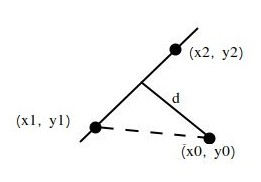
\includegraphics[width=0.4\textwidth]{dlugoscPktOdProstej}
\source{Na podstawie mathworld.wolfram.com}
\end{figure}


\begin{equation} \label{eq:distancePointLineal}
d = \frac{| (x_2 - x_1)(y_1 - y_0) - (x_1 - x_0)(y_2 - y_1) |}{\sqrt{(x_2 - x_1)^2 + (y_2 - y_1)^2}}
\end{equation}\newline

Rezultatem wdrożenia wzoru \ref{eq:distancePointLineal} do programu, są:
\begin{itemize}
\item na niebiesko zaznaczone drogi, na których znajdują się przejścia dla pieszych
\item znakiem ''D-6'' zostały oznaczone przejścia dla pieszysz
\end{itemize} 
Wynik został przedstawiony na Rys. \ref{sec:PrzejscieDrogi}:

\begin{figure}[h]
\caption{Drogi na których znajdują się przejścia dla pieszych.}
\label{sec:PrzejscieDrogi}
\centering
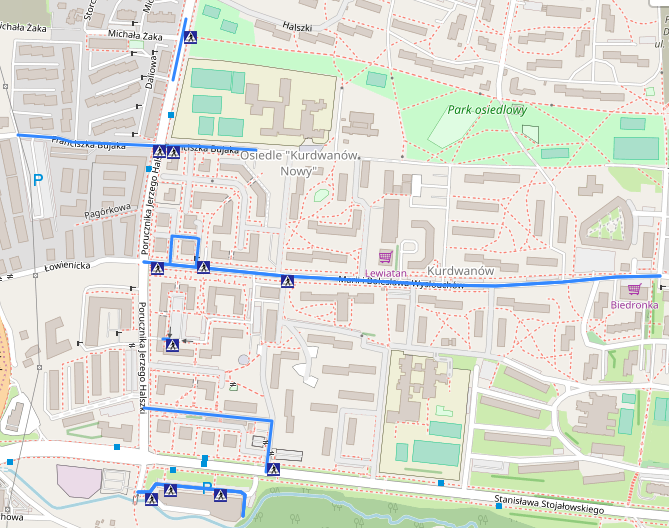
\includegraphics[width=0.8\textwidth]{PrzejscieDrogi}
\end{figure}


\newpage
\section{Liczba pasów ruchu}
\label{sec:zakręty}

\newpage
\section{Typ nawierzchni}
\label{sec:zakręty}

\newpage
\section{Rodzaj drogi}
\label{sec:zakręty}

\newpage
\section{Płynna zmiana prędkości pojazdów}
\label{sec:zakręty}

\newpage
\section{Przejazdy kolejowe}
\label{sec:zakręty}

\newpage
\section{Historia wypadków}
\label{sec:zakręty}

